\documentclass{ximera}

 

\usepackage{epsfig}

\graphicspath{
  {./}
  {figures/}
}

\usepackage{morewrites}
\makeatletter
\newcommand\subfile[1]{%
\renewcommand{\input}[1]{}%
\begingroup\skip@preamble\otherinput{#1}\endgroup\par\vspace{\topsep}
\let\input\otherinput}
\makeatother

\newcommand{\includeexercises}{\directlua{dofile("/home/jim/linearAlgebra/laode/exercises.lua")}}

%\newcounter{ccounter}
%\setcounter{ccounter}{1}
%\newcommand{\Chapter}[1]{\setcounter{chapter}{\arabic{ccounter}}\chapter{#1}\addtocounter{ccounter}{1}}

%\newcommand{\section}[1]{\section{#1}\setcounter{thm}{0}\setcounter{equation}{0}}

%\renewcommand{\theequation}{\arabic{chapter}.\arabic{section}.\arabic{equation}}
%\renewcommand{\thefigure}{\arabic{chapter}.\arabic{figure}}
%\renewcommand{\thetable}{\arabic{chapter}.\arabic{table}}

%\newcommand{\Sec}[2]{\section{#1}\markright{\arabic{ccounter}.\arabic{section}.#2}\setcounter{equation}{0}\setcounter{thm}{0}\setcounter{figure}{0}}

\newcommand{\Sec}[2]{\section{#1}}

\setcounter{secnumdepth}{2}
%\setcounter{secnumdepth}{1} 

%\newcounter{THM}
%\renewcommand{\theTHM}{\arabic{chapter}.\arabic{section}}

\newcommand{\trademark}{{R\!\!\!\!\!\bigcirc}}
%\newtheorem{exercise}{}

\newcommand{\dfield}{{\sf dfield9}}
\newcommand{\pplane}{{\sf pplane9}}

\newcommand{\EXER}{\section*{Exercises}}%\vspace*{0.2in}\hrule\small\setcounter{exercise}{0}}
\newcommand{\CEXER}{}%\vspace{0.08in}\begin{center}Computer Exercises\end{center}}
\newcommand{\TEXER}{} %\vspace{0.08in}\begin{center}Hand Exercises\end{center}}
\newcommand{\AEXER}{} %\vspace{0.08in}\begin{center}Hand Exercises\end{center}}

% BADBAD: \newcommand{\Bbb}{\bf}

\newcommand{\R}{\mbox{$\Bbb{R}$}}
\newcommand{\C}{\mbox{$\Bbb{C}$}}
\newcommand{\Z}{\mbox{$\Bbb{Z}$}}
\newcommand{\N}{\mbox{$\Bbb{N}$}}
\newcommand{\D}{\mbox{{\bf D}}}
\usepackage{amssymb}
%\newcommand{\qed}{\hfill\mbox{\raggedright$\square$} \vspace{1ex}}
%\newcommand{\proof}{\noindent {\bf Proof:} \hspace{0.1in}}

\newcommand{\setmin}{\;\mbox{--}\;}
\newcommand{\Matlab}{{M\small{AT\-LAB}} }
\newcommand{\Matlabp}{{M\small{AT\-LAB}}}
\newcommand{\computer}{\Matlab Instructions}
\newcommand{\half}{\mbox{$\frac{1}{2}$}}
\newcommand{\compose}{\raisebox{.15ex}{\mbox{{\scriptsize$\circ$}}}}
\newcommand{\AND}{\quad\mbox{and}\quad}
\newcommand{\vect}[2]{\left(\begin{array}{c} #1_1 \\ \vdots \\
 #1_{#2}\end{array}\right)}
\newcommand{\mattwo}[4]{\left(\begin{array}{rr} #1 & #2\\ #3
&#4\end{array}\right)}
\newcommand{\mattwoc}[4]{\left(\begin{array}{cc} #1 & #2\\ #3
&#4\end{array}\right)}
\newcommand{\vectwo}[2]{\left(\begin{array}{r} #1 \\ #2\end{array}\right)}
\newcommand{\vectwoc}[2]{\left(\begin{array}{c} #1 \\ #2\end{array}\right)}

\newcommand{\ignore}[1]{}


\newcommand{\inv}{^{-1}}
\newcommand{\CC}{{\cal C}}
\newcommand{\CCone}{\CC^1}
\newcommand{\Span}{{\rm span}}
\newcommand{\rank}{{\rm rank}}
\newcommand{\trace}{{\rm tr}}
\newcommand{\RE}{{\rm Re}}
\newcommand{\IM}{{\rm Im}}
\newcommand{\nulls}{{\rm null\;space}}

\newcommand{\dps}{\displaystyle}
\newcommand{\arraystart}{\renewcommand{\arraystretch}{1.8}}
\newcommand{\arrayfinish}{\renewcommand{\arraystretch}{1.2}}
\newcommand{\Start}[1]{\vspace{0.08in}\noindent {\bf Section~\ref{#1}}}
\newcommand{\exer}[1]{\noindent {\bf \ref{#1}}}
\newcommand{\ans}{}
\newcommand{\matthree}[9]{\left(\begin{array}{rrr} #1 & #2 & #3 \\ #4 & #5 & #6
\\ #7 & #8 & #9\end{array}\right)}
\newcommand{\cvectwo}[2]{\left(\begin{array}{c} #1 \\ #2\end{array}\right)}
\newcommand{\cmatthree}[9]{\left(\begin{array}{ccc} #1 & #2 & #3 \\ #4 & #5 &
#6 \\ #7 & #8 & #9\end{array}\right)}
\newcommand{\vecthree}[3]{\left(\begin{array}{r} #1 \\ #2 \\
#3\end{array}\right)}
\newcommand{\cvecthree}[3]{\left(\begin{array}{c} #1 \\ #2 \\
#3\end{array}\right)}
\newcommand{\cmattwo}[4]{\left(\begin{array}{cc} #1 & #2\\ #3
&#4\end{array}\right)}

\newcommand{\Matrix}[1]{\ensuremath{\left(\begin{array}{rrrrrrrrrrrrrrrrrr} #1 \end{array}\right)}}

\newcommand{\Matrixc}[1]{\ensuremath{\left(\begin{array}{cccccccccccc} #1 \end{array}\right)}}



\renewcommand{\labelenumi}{\theenumi)}
\newenvironment{enumeratea}%
{\begingroup
 \renewcommand{\theenumi}{\alph{enumi}}
 \renewcommand{\labelenumi}{(\theenumi)}
 \begin{enumerate}}
 {\end{enumerate}\endgroup}



\newcounter{help}
\renewcommand{\thehelp}{\thesection.\arabic{equation}}

%\newenvironment{equation*}%
%{\renewcommand\endequation{\eqno (\theequation)* $$}%
%   \begin{equation}}%
%   {\end{equation}\renewcommand\endequation{\eqno \@eqnnum
%$$\global\@ignoretrue}}

%\input{psfig.tex}

\author{Martin Golubitsky and Michael Dellnitz}

%\newenvironment{matlabEquation}%
%{\renewcommand\endequation{\eqno (\theequation*) $$}%
%   \begin{equation}}%
%   {\end{equation}\renewcommand\endequation{\eqno \@eqnnum
% $$\global\@ignoretrue}}

\newcommand{\soln}{\textbf{Solution:} }
\newcommand{\exercap}[1]{\centerline{Figure~\ref{#1}}}
\newcommand{\exercaptwo}[1]{\centerline{Figure~\ref{#1}a\hspace{2.1in}
Figure~\ref{#1}b}}
\newcommand{\exercapthree}[1]{\centerline{Figure~\ref{#1}a\hspace{1.2in}
Figure~\ref{#1}b\hspace{1.2in}Figure~\ref{#1}c}}
\newcommand{\para}{\hspace{0.4in}}

\renewenvironment{solution}{\suppress}{\endsuppress}

\ifxake
\newenvironment{matlabEquation}{\begin{equation}}{\end{equation}}
\else
\newenvironment{matlabEquation}%
{\let\oldtheequation\theequation\renewcommand{\theequation}{\oldtheequation*}\begin{equation}}%
  {\end{equation}\let\theequation\oldtheequation}
\fi

\makeatother


\title{*Markov Chains}

\begin{document}
\begin{abstract}
\end{abstract}
\maketitle


\label{S:TransitionApplied}

Markov chains provide an interesting and useful application of matrices and
linear algebra.  In this section we introduce Markov chains via some of the
theory and two examples.  The theory can be understood and applied to examples
using just the background in linear algebra that we have developed in this
chapter.


\subsection*{An Example of Cats}

Consider the four room apartment pictured in Figure~\ref{F:apart}.  One way
passages between the rooms are indicated by arrows.  For example, it is
possible to go from room~1 directly to any other room, but when in room~3
it is possible to go only to room~4.

\begin{figure}[htb]
        \centerline{%
        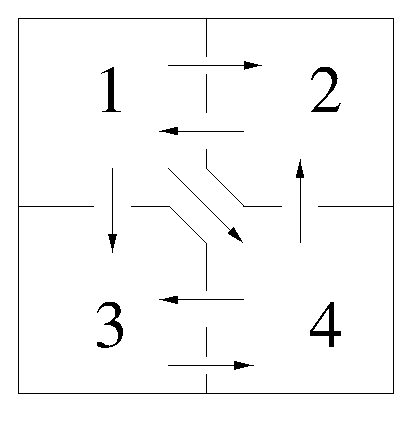
\psfig{file=../figures/apart.eps,width=3.2in}}
        \caption{Schematic design of apartment passages.}
        \label{F:apart}
\end{figure}

Suppose that there is a cat in the apartment and that at each hour the cat is
asked to move from the room that it is in to another.  True to form, however,
the cat chooses with equal probability to stay in the room for another hour
or to move through one of the allowed passages.  Suppose that we let $p_{ij}$
be the probability that the cat will move from room~$i$ to room~$j$; in
particular, $p_{ii}$ is the probability that the cat will stay in room~$i$.
For example, when the cat is in room~1, it has four choices  --- it can
stay in room~1 or move to any of the other rooms.  Assuming that each of
these choices is made with equal probability, we see that
\[
p_{11} = \frac{1}{4} \qquad p_{12} = \frac{1}{4} \qquad p_{13} =
\frac{1}{4} \qquad p_{14} = \frac{1}{4}.
\]
It is now straightforward to verify that
\[
p_{21} = \frac{1}{2} \qquad p_{22} = \frac{1}{2} \qquad p_{23} = 0
\qquad p_{24} = 0
\]
\[
p_{31} = 0 \qquad p_{32} = 0 \qquad p_{33} =
\frac{1}{2} \qquad p_{34} = \frac{1}{2}
\]
\[
p_{41} = 0 \qquad p_{42} = \frac{1}{3} \qquad p_{43} =
\frac{1}{3} \qquad p_{44} = \frac{1}{3}.
\]

Putting these probabilities together yields the
{\em transition matrix}\index{matrix!transition}:
\begin{matlabEquation} \label{E:Pexamp}
P = \left(\begin{array}{cccc}
\frac{1}{4} & \frac{1}{4} & \frac{1}{4} & \frac{1}{4} \\
\half & \half & 0 & 0 \\
 0 & 0 & \half & \half\\
0 & \frac{1}{3} & \frac{1}{3} & \frac{1}{3}
\end{array}\right)
\end{matlabEquation}
This transition matrix has the properties that all entries are nonnegative
and that the entries in each row sum to $1$.

\subsubsection*{Three Basic Questions}

Using the transition matrix $P$, we discuss the answers to three questions:
\begin{enumerate}
\item[(A)] What is the probability that a cat starting in room~$i$ will
be in room~$j$ after exactly $k$ steps?  We call the movement that occurs
after each hour a {\em step\/}.
\item[(B)] Suppose that we put 100 cats in the apartment with some initial
distribution of cats in each room.  What will the distribution of cats
look like after a large number of steps?
\item[(C)] Suppose that a cat is initially in room~$i$ and takes a large
number of steps.  For how many of those steps will the cat be expected to
be in room~$j$?
\end{enumerate}

\subsubsection*{A Discussion of Question (A)}

We begin to answer Question (A) by determining the probability that the
cat moves from room~1 to room~4 in two steps.  We denote this probability
by $p_{14}^{(2)}$ and compute
\begin{equation} \label{E:prob14}
p_{14}^{(2)} = p_{11}p_{14} + p_{12}p_{24} + p_{13}p_{34} + p_{14}p_{44};
\end{equation}
that is, the probability is the sum of the probabilities that the cat will
move from room~$1$ to each room~$i$ and then from room~$i$ to room~4.  In
this case the answer is:
\[
p_{14}^{(2)} = \frac{1}{4}\times\frac{1}{4} + \frac{1}{4}\times0 +
\frac{1}{4}\times\frac{1}{2} + \frac{1}{4}\times\frac{1}{3} =
\frac{13}{48} \approx 0.27\;.
\]
It follows from \eqref{E:prob14} and the definition of matrix multiplication
that $p_{14}^{(2)}$ is just the $(1,4)^{th}$ entry in the matrix $P^2$.  An
induction argument shows that the probability of the cat moving from
room~$i$ to room~$j$ in $k$ steps is precisely the $(i,j)^{th}$ entry in the
matrix $P^k$ --- which answers Question (A).  In particular, we can answer the
question: What is the probability that the cat will move from room~4 to room~3
in four steps?  Using \Matlab the answer is given by typing {\tt e4\_10\_1} to
recall the matrix $P$ and then typing
\begin{verbatim}
P4 = P^4;
P4(4,3)
\end{verbatim}
obtaining
\begin{verbatim}
ans =
    0.2728
\end{verbatim}

\subsubsection*{A Discussion of Question (B)}

We answer Question (B) in two parts: first we compute a formula for
determining the number of cats that are expected to be in room~$i$ after $k$
steps, and second we explore that formula numerically for large $k$.  We
begin by supposing that 100 cats are distributed in the rooms according to
the initial vector $V_0=(v_1,v_2,v_3,v_4)^t$; that is, the number of cats
initially in room~$i$ is $v_i$.  Next, we denote the number of cats that are
expected to be in room~$i$ after $k$ steps by $v_i^{(k)}$.  For example, we
determine how many cats we expect to be in room~2 after one step.  That
number is:
\begin{equation} \label{E:probt2}
v_2^{(1)}=p_{12}v_1 + p_{22}v_2 + p_{32}v_3 + p_{42}v_4;
\end{equation}
that is, $v_2^{(1)}$ is the sum of the proportion of cats in each room~$i$
that are expected to migrate to room~2 in one step.  In this case, the answer
is:
\[
\frac{1}{4}v_1 + \frac{1}{2}v_2 + \frac{1}{3}v_4.
\]
It now follows from \eqref{E:probt2}, the definition of the transpose of a
matrix, and the definition of matrix multiplication that $v_2^{(1)}$ is
the $2^{nd}$ entry in the vector $P^tV_0$.  Indeed, it follows by induction
that $v_i^{(k)}$ is the $i^{th}$ entry in the vector $(P^t)^kV_0$ which
answers the first part of Question (B).

We may rephrase the second part of Question (B) as follows.  Let
\[
V_k = (v_1^{k},v_2^{k},v_3^{k},v_4^{k})^t = (P^t)^kV_0.
\]
Question (B) actually asks: What will the vector $V_k$ look like for
large $k$.  To answer that question we need some results about matrices
like the matrix $P$ in \eqref{E:Pexamp}.  But first we explore the answer to
this question numerically using \Matlabp.

Suppose, for example, that the initial vector is
\begin{matlabEquation}\label{MATLAB:9}
V_0 =\left(\begin{array}{c} 2 \\ 43 \\ 21 \\ 34 \end{array}\right).
\end{matlabEquation}
Typing {\tt e4\_10\_1} and {\tt e4\_10\_4} enters the matrix $P$ and the
initial vector $V_0$ into \Matlabp.  To compute $V_{20}$, the distribution
of cats after $20$ steps, type
\begin{verbatim}
Q=P'
V20 = Q^(20)*V0
\end{verbatim}
and obtain
\begin{verbatim}
V20 =
   18.1818
   27.2727
   27.2727
   27.2727
\end{verbatim}
Thus, after rounding to the nearest integer, we expect $27$ cats to be in
each of rooms~2,3 and 4 and 18 cats to be in room~1 after $20$ steps.  In
fact, the vector $V_{20}$
has a remarkable feature.  Compute {\tt Q*V20} in \Matlab and see that
$V_{20} = P^tV_{20}$; that is, $V_{20}$ is, to within four digit numerical
precision, an eigenvector of $P^t$ with eigenvalue equal to $1$.  This
computation was not a numerical accident, as we now describe.  Indeed,
compute $V_{20}$ for several initial distributions $V_0$ of cats and see that
the answer will always be the same --- up to four digit accuracy.

\subsubsection*{A Discussion of Question (C)}

Suppose there is just one cat in the apartment; and we ask how many times that
cat is expected to visit room~3 in $100$ steps.  Suppose the cat starts in
room~1; then the initial distribution of cats is one cat in room~1 and zero
cats in any of the other rooms.  So $V_0=e_1$.  In our discussion of
Question (B) we saw that the $3^{rd}$ entry in $(P^t)^kV_0$ gives the
probability $c_k$ that the cat will be in room~3 after $k$ steps.

In the extreme, suppose that the probability that the cat will be in room~3 is
$1$ for each step $k$.  Then the fraction of the time that the cat is in room~3
is
\[
(1 + 1 + \cdots + 1)/100 = 1.
\]
In general, the fraction of the time $f$ that the cat will be in room~3
during a span of $100$ steps is
\[
f = \frac{1}{100}(c_1 + c_2 +\cdots + c_{100}).
\]
Since $c_k = (P^t)^kV_0$, we see that
\begin{equation}  \label{E:f}
f = \frac{1}{100}(P^tV_0 + (P^t)^2V_0 + \cdots + (P^t)^{100}V_0).
\end{equation}

So, to answer Question (C), we need a way to sum the expression for $f$
in \eqref{E:f}, at least approximately.  This is not an easy task --- though
the answer itself is easy to explain.  Let $V$ be the eigenvector of $P^t$
with eigenvalue $1$ such that the sum of the entries in $V$ is $1$.  The
answer is: $f$ is approximately equal to $V$.  See Theorem~\ref{T:ergodic}
for a more precise statement.

In our previous calculations the vector $V_{20}$ was seen to be (approximately)
an eigenvector of $P^t$ with eigenvalue $1$.  Moreover the sum of the entries
in $V_{20}$ is precisely $100$.  Therefore, we normalize $V_{20}$ to get $V$
by setting
\[
V =\frac{1}{100}V_{20}.
\]
So, the fraction of time that the cat spends in room~3 is $f\approx 0.2727$.
Indeed, we expect the cat to spend approximately $27\%$ of its time in rooms
2,3,4 and about $18\%$ of its time in room~1.

\subsection*{Markov Matrices}

We now abstract the salient properties of our cat example.  A
{\em Markov chain\/}\index{Markov chain} is a system with a
finite number of states labeled
$1$,\dots,$n$ along with probabilities $p_{ij}$ of moving from site $i$ to
site $j$ in a single step.  The Markov assumption is that these probabilities
depend only on the site that you are in and not on how you got there.  In our
example, we assumed that the probability of the cat moving from say room~2 to
room~4 did not depend on how the cat got to room~2 in the first place.

We make a second assumption: there is a $k$ such that it is possible to move
from any site $i$ to any site $j$ in exactly $k$ steps.  This assumption is
{\em not\/} valid for general Markov chains, though it is valid for the cat
example, since it is possible to move from any room to any other room in that
example in exactly three steps.  (It takes a minimum of three steps to get
from room~3 to room~1 in the cat example.)  To simplify our discussion we
include this assumption in our definition of a Markov chain.

\begin{definition}  \label{D:Markov}
{\em Markov matrices\/}\index{matrix!Markov} are square matrices
$P$ such that
\begin{enumerate}
\item[(a)]  all entries in $P$ are nonnegative,
\item[(b)]  the entries in each row of $P$ sum to $1$, and
\item[(c)]  there is a positive integer $k$ such that all of the entries
	in $P^k$ are positive.
\end{enumerate}
\end{definition}

It is straightforward to verify that parts (a) and (b) in the definition of
Markov matrices are satisfied by the transition matrix
\[
P = \left(\begin{array}{ccc} p_{11} & \cdots & p_{1n} \\
	\vdots & \vdots & \vdots \\ p_{n1} & \cdots & p_{nn}
\end{array}\right)
\]
of a Markov chain.  To verify part (c) requires further discussion.

\begin{proposition}   \label{T:Markoveasy}
Let $P$ be a transition matrix\index{matrix!transition} for a
Markov chain\index{Markov chain}.
\begin{enumerate}
\item[(a)]  The probability of moving from site $i$ to site $j$ in exactly
$k$ steps is the $(i,j)^{th}$ entry in the matrix $P^k$.
\item[(b)]  The expected number of individuals at site $i$ after exactly $k$
steps is the $i^{th}$ entry in the vector $V_k\equiv (P^t)^kV_0$.
\item[(c)]  $P$ is a Markov matrix\index{matrix!Markov}.
\end{enumerate}
\end{proposition}

\begin{proof} Only minor changes in our discussion of the cat example proves parts
(a) and (b) of the proposition.

(c) The assumption that it is possible to move from each site~$i$ to each
site~$j$ in exactly $k$ steps means that the $(i,j)^{th}$ entry of $P^k$ is
positive.  For that $k$, all of the entries of $P^k$ are positive.  In the
cat example, all entries of $P^3$ are positive.  \end{proof}

Proposition~\ref{T:Markoveasy} gives the answer to Question (A) and the first
part of Question (B) for general Markov chains.

Let $v_i^{(0)}\ge 0$ be the number of individuals initially at site $i$, and
let $V_0=(v_1^{(0)},\ldots,v_n^{(0)})^t$.  The total number of individuals
in the initial population is:
\[
\#(V_0) = v_1^{(0)} + \cdots + v_n^{(0)}.
\]

\begin{theorem}  \label{T:Markov}
Let $P$ be a Markov matrix\index{matrix!Markov}.  Then
\begin{enumerate}
\item[(a)]  $\#(V_k)=\#(V_0)$; that is, the number of individuals after $k$
time steps is the same as the initial number.
\item[(b)]  $\dps V = \lim_{k\to\infty}V_k$ exists and $\#(V)=\#(V_0)$.
\item[(c)]  $V$ is an eigenvector of $P^t$ with eigenvalue equal to $1$.
\end{enumerate}
\end{theorem}

\begin{proof}  (a) By induction it is sufficient to show that $\#(V_1)=\#(V_0)$.  We
do
this by calculating from $V_1 = P^tV_0$ that
\begin{eqnarray*}
\#(V_1) & = & v_1^{(1)} + \cdots + v_n^{(1)}\\
& = & (p_{11}v_1^{(0)} + \cdots + p_{n1}v_n^{(0)}) + \cdots +
	(p_{1n}v_1^{(0)} + \cdots + p_{nn}v_n^{(0)}) \\
& = & (p_{11}+ \cdots + p_{1n})v_1^{(0)}  + \cdots +
	(p_{n1} + \cdots + p_{nn})v_n^{(0)} \\
& = & v_1^{(0)}  + \cdots + v_n^{(0)}
\end{eqnarray*}
since the entries in each row of $P$ sum to $1$.  Thus $\#(V_1)=\#(V_0)$, as
claimed.

(b)	The hard part of this theorem is proving that the limiting vector $V$
exists; we give a proof of this fact in Chapter~\ref{C:HDeigenvalues},
Theorem~\ref{T:convergetoeig}.  Once $V$ exists it follows directly from (a)
that $\#(V)=\#(V_0)$.

(c)   	Just calculate that
\begin{align*}
P^tV &= P^t(\lim_{k\to\infty}V_k) = P^t(\lim_{k\to\infty}(P^t)^kV_0) \\
&= \lim_{k\to\infty}(P^t)^{k+1}V_0 = \lim_{k\to\infty}(P^t)^kV_0 = V,
\end{align*}
which proves (c).   \end{proof}

Theorem~\ref{T:Markov}(b) gives the answer to the second part of Question (B)
for general Markov chains.  Next we discuss Question (C).

\begin{theorem} \label{T:ergodic}
Let $P$ be a Markov matrix\index{matrix!Markov}.
Let $V$ be the eigenvector of $P^t$ with
eigenvalue $1$ and $\#(V)=1$.  Then after a large number of steps $N$ the
expected number of times an individual will visit site~$i$ is $Nv_i$ where
$v_i$ is the $i^{th}$ entry in $V$.
\end{theorem}

\begin{proof}[Sketch] In our discussion of Question (C) for the
cat example, we explained why the fraction $f_N$ of time that an individual
will visit site~$j$ when starting initially at site~$i$ is the $j^{th}$ entry
in the sum
\[
f_N = \frac{1}{N}(P^t + (P^t)^2 + \cdots + (P^t)^N)e_i.
\]
See \eqref{E:f}.  The proof of this theorem involves being able to calculate
the limit of $f_N$ as $N\to\infty$.  There are two main ideas.  First, the
limit of the matrix $(P^t)^N$ exists as $N$ approaches infinity --- call that
limit $Q$.  Moreover, $Q$ is a matrix all of whose columns equal $V$.
Second, for large $N$, the sum
\[
P^t + (P^t)^2 + \cdots + (P^t)^N \approx Q + Q + \cdots + Q = NQ,
\]
so that the limit of the $f_N$ is $Qe_i=V$.

The verification of these statements is beyond the scope of this text.
For those interested, the idea of the proof of the second part is roughly the
following.  Fix $k$ large enough so that $(P^t)^k$ is close to $Q$.  Then when
$N$ is large, much larger than $k$, the sum of the first $k$ terms in the
series is nearly zero.  \end{proof}


Theorem~\ref{T:ergodic} gives the answer to Question (C) for a general Markov
chain.  It follows from Theorem~\ref{T:ergodic} that for Markov chains the
amount of time that an individual spends in room~$i$ is independent of the
individual's initial room --- at least after a large number of steps.

A complete proof of this theorem relies on a result known as the {\em ergodic
theorem}.
Roughly speaking, the ergodic theorem relates space averages
with time averages.   To see how this point is relevant, note that Question (B)
deals with the issue of how a large number of individuals will be distributed
in space after a large number of steps, while Question (C) deals with the
issue of how the path of a single individual will be distributed in time after
a large number of steps.

\subsubsection*{An Example of Umbrellas}

This example focuses on the utility of answering Question (C) and reinforces
the fact that results in Theorem~\ref{T:Markov} have the second
interpretation given in Theorem~\ref{T:ergodic}.

Consider the problem of a man with four umbrellas.  If it is raining in the
morning when the man is about to leave for his office, then the man takes an
umbrella from home to office, assuming that he has an umbrella at home.  If it
is raining in the afternoon, then the man takes an umbrella from office to
home, assuming that he has an umbrella in his office.  Suppose that the
probability that it will rain in the morning is $p=0.2$ and the probability
that it will rain in the afternoon is $q=0.3$, and these probabilities are
independent.  What percentage of days will the man get wet going from home
to office; that is, what percentage of the days will the man be at home on a
rainy morning with all of his umbrellas at the office?

There are five states in the system depending on the number of umbrellas that
are at home.  Let $s_i$ where $0\leq i\leq 4$ be the state with $i$ umbrellas
at home and $4-i$ umbrellas at work.  For example, $s_2$ is the state of
having two umbrellas at home and two at the office.  Let $P$ be the
$5\times 5$ transition matrix of state changes from morning to afternoon and
$Q$ be the $5\times 5$ transition matrix of state changes from afternoon to
morning.  For example, the probability $p_{23}$ of moving from site $s_2$ to
site $s_3$ is $0$, since it is not possible to have more umbrellas at home
after going to work in the morning.  The probability $q_{23}=q$, since the
number of umbrellas at home will increase by one only if it is raining in the
afternoon.  The transition probabilities between all states are given in the
following transition matrices:
\[
P = \left(\begin{array}{ccccc} 1 & 0 & 0 & 0 & 0 \\
  p & 1-p & 0 & 0 & 0 \\ 0 & p & 1-p & 0 & 0 \\ 0 & 0 & p & 1-p & 0 \\
            0 & 0 & 0 & p & 1-p \end{array}\right);\]
      \[
Q = \left(\begin{array}{ccccc} 1-q & q & 0 & 0 & 0 \\
  0 & 1-q & q & 0 & 0 \\ 0 & 0 & 1-q & q & 0 \\ 0 & 0 & 0 & 1-q & q \\
 0 & 0 & 0 & 0 & 1 \end{array}\right)
\]
Specifically,
\begin{matlabEquation}\label{MATLAB:10}
P =
\left(\begin{array}{ccccc} 1 & 0 & 0 & 0 & 0 \\
  0.2 & 0.8 & 0 & 0 & 0 \\ 0 & 0.2 & 0.8 & 0 & 0 \\ 0 & 0 & 0.2 & 0.8 & 0 \\
        0 & 0 & 0 & 0.2 & 0.8 \end{array}\right)
  \end{matlabEquation}
\begin{equation*}
Q =
\left(\begin{array}{ccccc} 0.7 & 0.3 & 0 & 0 & 0 \\
  0 & 0.7 & 0.3 & 0 & 0 \\ 0 & 0 & 0.7 & 0.3 & 0 \\ 0 & 0 & 0 & 0.7 & 0.3 \\
 0 & 0 & 0 & 0 & 1 \end{array}\right)
\end{equation*}

The transition matrix\index{matrix!transition} $M$ from
moving from state $s_i$ on one morning to
state $s_j$ the next morning is just $M=PQ$.  We can compute this matrix
using \Matlab by typing
\begin{verbatim}
e4_10_6
M = P*Q
\end{verbatim}
obtaining
\begin{verbatim}
M =
    0.7000    0.3000         0         0         0
    0.1400    0.6200    0.2400         0         0
         0    0.1400    0.6200    0.2400         0
         0         0    0.1400    0.6200    0.2400
         0         0         0    0.1400    0.8600
\end{verbatim}
It is easy to check using \Matlab that all entries in the matrix $M^4$ are
nonzero.  So $M$ is a Markov matrix\index{matrix!Markov} and we can use
Theorem~\ref{T:ergodic}
to find the limiting distribution of states.  Start with some initial
condition like $V_0=(0,0,1,0,0)^t$ corresponding to the state in which two
umbrellas are at home and two at the office.  Then compute the vectors
$V_k=(M^t)^kV_0$ until arriving at an eigenvector of $M^t$ with eigenvalue 1.
For example, $V_{70}$ is computed by typing \verb+V70 = M'^(70)*V0+ and
obtaining
\begin{verbatim}
V70 =
    0.0419
    0.0898
    0.1537
    0.2633
    0.4512
\end{verbatim}
We interpret $V\approx V_{70}$ in the following way.  Since $v_1$ is
approximately $.042$, it follows that for approximately $4.2\%$ of all steps 
the umbrellas are in state $s_0$.  That is, approximately $4.2\%$ of all days 
there are no umbrellas at home.  The probability that it will rain in the 
morning on one of those days is $0.2$.  Therefore, the probability of being 
at home in the morning when it is raining without any umbrellas is 
approximately $0.008$.





\EXER

\includeexercises



\end{document}

%%% Local Variables:
%%% mode: latex
%%% TeX-master: "../linearAlgebra"
%%% End:
